\documentclass[letterpaper,11pt]{article}
\usepackage{graphicx}
\usepackage[font=small,labelfont=bf]{caption}
\usepackage{amssymb}
\usepackage{amsmath}
\usepackage{indentfirst}
\usepackage[utf8]{inputenc}
\usepackage{titling}
\usepackage[ruled,linesnumbered]{algorithm2e}
\usepackage{tabu}
\usepackage[left=2cm, right=2cm, top=1cm]{geometry}
\usepackage{tikz}
\usepackage{listings}
\graphicspath{{images/}}
\usepackage[pdftex,
    pdfauthor={Ignacio Martinez Hernandez},
    pdftitle={Tarea 5},
    pdfsubject={Modelos Discretos},
    ]{hyperref}

\pretitle{\begin{center}\Huge\bfseries}
\posttitle{\par\end{center}}
\predate{\begin{flushright}\Large}
\postdate{\end{flushright}}
\preauthor{\begin{flushright}\Large}
\postauthor{\end{flushright}}

\title{Informe Tarea 5 \\ \vskip 0.5em Grafos}
\date{\vspace{-8ex}}


\lstset{language=C++,
                basicstyle=\ttfamily,
                keywordstyle=\color{blue}\ttfamily,
                stringstyle=\color{red}\ttfamily,
                commentstyle=\color{green}\ttfamily,
                morecomment=[l][\color{magenta}]{\#},
                xleftmargin=-80pt
}

\author
{
    Fecha: \today \\
    Ignacio Martínez Hernández \\ 
    e-mail: \href{mailto:imartinez17@alumnos.utalca.cl}{imartinez17@alumnos.utalca.cl} \\ 
}
\begin{document}  

\vbox
{
    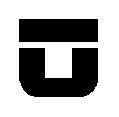
\includegraphics[]{utalca.eps}.
    \rlap{\kern 4mm \lower -9.5mm \hbox to0pt{{\Large \sc Universidad~~de~~Talca}\hfill}}%
    \rlap{\kern 4mm \lower -5mm \hbox to0pt{\Large \sc Facultad~~de~~Ingenier\'ia\hfill}}%
    \rlap{\kern 4mm \lower -1mm \hbox to0pt{%
    {\large \sc Departamento~~de~~Ciencias~~de~~la~~Computaci\'on}\hfill}}%      
    \maketitle
}   

\section{Introducción}
    En este informe, implementaré los algoritmos de Kruskal para la construcción del árbol cobertor mínimo y  de Dijkstra para el cómputo de caminos más cortos, con el fin de analizar su comportamiento.
\section{Análisis del problema}
    Para poder implementar los algoritmos del árbol cobertor mínimo y cómputo de caminos más cortos, primero es importante tener un grafo euclidiano conexo. Por eso, lo primero que se hizo fue la implementación de un algoritmo simple en C++ que creará un grafo totalmente aleatorio dado los parámetros ingresados en un espacio euclidiano dentro de un cuadrado unitario $[0,1] \times [0,1]$ y luego convertirla en su representación de Lista de Adyacencia para que Kruskal o Dijkstra lo utilicen.
    Después se pasó a implementar los algoritmos utilizando como guía \href{https://users.dcc.uchile.cl/~raparede/publ/08PhDthesis.pdf}{Grafos para búsqueda en espacios métricos}. 
\section{Solución del problema}

    \subsection{Creación del grafo}
        \subsubsection{Algoritmo de solución}
            \begin{itemize}
                \item Se calculó el número de conexiones que se utilizarán con la fórmula $densidad \cdot (\frac{n \cdot (n-1)}{2})$.
                \item Se calcula $\Delta = \frac{1}{n}$ el cual se usa para generar un arreglo con distancias uniformes en las coordenadas $x,y$.
                \item Se hace un shuffle a los arreglos y luego se emparejan creando un nuevo arreglo con puntos aleatorios en $[0,1] \times [0,1]$.
                \item Se crea una matriz de adyacencia la cual va a contener -1 (indicando que no existe conexión) y 0 en sus diagonales (sólo para indicar que la distancia del nodo a si mismo es 0).   
                \item En la matriz de adyacencia se le asignan conexiones para que sea conexa utilizando el arreglo que contiene las coordenadas.
                \item Después de tener una matriz de adyacencia conexa se generan más conexiones para asegurar la densidad.
                \item Por último, la matriz de adyacencia se convierte a una lista de adyacencia para luego ser utilizada por los respectivos algoritmos.
            \end{itemize}

        \subsubsection{Implementación}
        \begin{algorithm}[H]
            \SetKwInOut{Input}{input}
            \Input{$n$ $densidad$}
            $edgesN \gets densidad \cdot (\frac{n \cdot (n-1)}{2})$

            $nodes , x , y, w \gets \emptyset$

            $\Delta \gets \frac{1}{n}$

            \For{$i\gets0$ \textbf{to} $n$}
            {
                $x \gets x \cup \Delta \cdot (i+1)$
                
                $y \gets y \cup \Delta \cdot (i+1)$
            }
            \textbf{suffle$(x)$} , \textbf{suffle$(y)$}

            \For{$i\gets0$ \textbf{to} $n$}
            {
                $nodes \gets nodes \cup (x_i , y_i)$
            }

            \For{$i\gets0$ \textbf{to} $n$}
            {
                \For{$j\gets0$ \textbf{to} $n$}
                {
                    \eIf{$i == j$}
                    {
                        $w_{i,j} \gets 0$
                    } 
                    {
                        $w_{i,j} \gets 1$
                    }
                }                
            }

            \For{$i\gets0$ \textbf{to} $n-1$}
            {
                $w_{i,i+1} \gets w_{i+1,i} \gets $\textbf{distance$(nodes_i, nodes_{i+1})$}
            }

            \While{$i < edgesN$}
            {
                $x' \gets $ \textbf{random()}

                $y' \gets $ \textbf{random()}

                \If{$x' \neq y' \land w_{x',y'} < 0$}
                {
                    $w_{x',y'} \gets w_{y',x'} \gets $\textbf{distance$(nodes_{x'}, nodes_{y'})$}
                    
                    $w_{x',y'} \gets w_{y',x'} \gets 0$
                }
            }


        \end{algorithm}

    \newpage
    \subsection{Kruskal}
        \subsubsection{Algoritmo de solución}
        
            Aquí una simple representación de como funcionaría el algoritmo:
            
            \begin{table}[h]
                \centering
                \begin{tabu}to \textwidth {X[c]X[c]}
                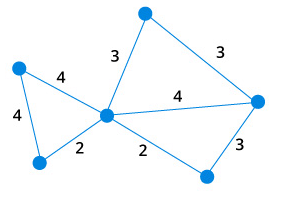
\includegraphics[width=45mm]{kruskal0.png}\captionof{figure}{Comenzar con un grafo conexo.} &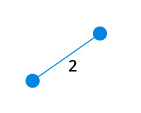
\includegraphics[width=45mm]{kruskal1.png}\captionof{figure}{Seleccionar la arista con menor peso.} \\
                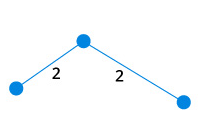
\includegraphics[width=45mm]{kruskal2.png}\captionof{figure}{Seleccionar la siguiente arista con menos peso.} &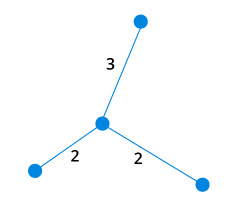
\includegraphics[width=45mm]{kruskal3.png}\captionof{figure}{Seleccionar la siguiente arista con menos peso que no genere un ciclo.} \\
                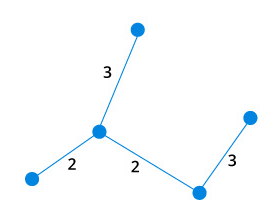
\includegraphics[width=45mm]{kruskal4.png}\captionof{figure}{Seleccionar la siguiente arista con menos peso.} &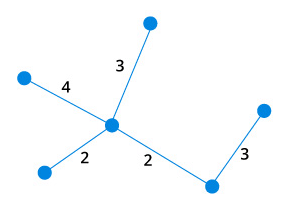
\includegraphics[width=45mm]{kruskal5.png}\captionof{figure}{Repetir hasta obtener el árbol cobertor mínimo.} \\
                \end{tabu}
            \end{table}

            Para implementar el algoritmo como se describió anteriormente se hizo lo siguiente:
            \begin{itemize}
                \item Se utilizó Union-Find, con el fin de consultar si se generaría un ciclo.
                \item La representación del grafo conexo (Lista de adyacencia), se pasó a una cola de prioridad (Lista de aristas) para poder obtener de manera rápida las aristas de menor peso.
                \item Y gracias a lo anterior al retirar una arista, utilizando Find se verifica que no formen un ciclo, de no ser así, se agrega y se aplica Union para actualizar.    
            \end{itemize}
                
        \subsubsection{Implementación}
        \begin{algorithm}[H]
            \SetKwInOut{Input}{input}
            \Input{Adjacency List $Adj$}
            $T \gets \emptyset$

            $weight \gets 0$

            UnionFind $C \gets \{\{v\}, v \in Adj_V \}$ //V = Vertex
            
            \textbf{heapify($Adj_E$)}

            \While{$|Adj_v| -1  > |Adj_E| > 0 $}
            {
                Edge $cur \gets Adj_E.$\textbf{extractMin}() // E = Edges

                \If{$C.$\textbf{find$(cur$.u$)$} $\neq C.$\textbf{find$(cur$.v$)$}}
                {
                    $T \gets T \cup cur$

                    $weight \gets weight + curr.$\textbf{weight}

                    $C.$\textbf{union$(u,v)$}
                }
            }
            \textbf{return} $T$
        \end{algorithm}

    \newpage
    \subsection{Dijkstra}
        \subsubsection{Algoritmo de solución}
            Aquí una simple representación de como funcionaría el algoritmo:
            
            \begin{table}[h]
                \centering
                \begin{tabu}to \textwidth {X[c]X[c]}
                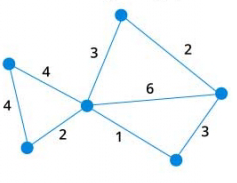
\includegraphics[width=45mm]{dijkstra0.png}\captionof{figure}{Comenzar con un grafo conexo.} &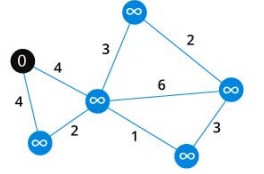
\includegraphics[width=45mm]{dijkstra1.png}\captionof{figure}{Escoger el nodo de inicio y asignar $\infty$ de distancia a los demás nodos.} \\
                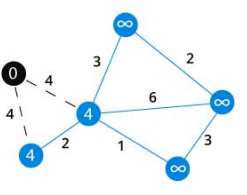
\includegraphics[width=45mm]{dijkstra2.png}\captionof{figure}{Ir a cada nodo adyacente del nodo y actualizar valores.} &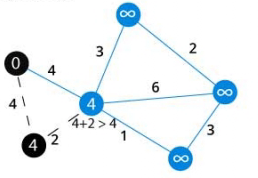
\includegraphics[width=45mm]{dijkstra3.png}\captionof{figure}{Si el camino del nodo adyacente es menor al nuevo camino, no se actualiza.} \\
                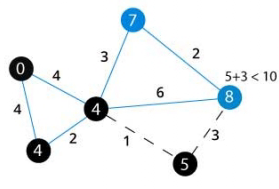
\includegraphics[width=45mm]{dijkstra4.png}\captionof{figure}{Después de cada iteración, se escoge el nodo no visitado con menos costo.} &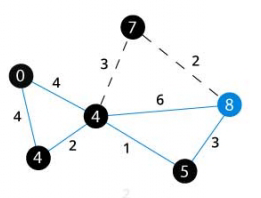
\includegraphics[width=45mm]{dijkstra5.png}\captionof{figure}{Repetir hasta haber visitado todos los nodos.} \\ 
                \end{tabu}
            \end{table}
            
            Para implementar el algoritmo como se describió anteriormente, se hizo lo siguiente:

            \begin{itemize}
                \item Se crearon dos arreglos, uno que contiene las distancias con $\infty$ y otro el camino hacia los nodos padre de cada nodo, éste nos ayuda a saber si ya fue visitado o no.
                \item Se creó una cola de prioridad donde se le fuerza la inserción de una tupla la cual contiene (peso , idNodo)  ordenando de menor a mayor, esto ayuda a escoger los posibles caminos a visitar con menor peso.
                \item Si el camino del nodo adyacente es menor al nuevo camino, se actualizan los datos de distancia y padre, agregando esta nueva información también a la cola de prioridad.
                \item Repetir hasta que la cola de prioridad esté vacía.
            \end{itemize}

        \subsubsection{Implementación}
        \begin{algorithm}[H]
            \SetKwInOut{Input}{input}
            \Input{Adjacency List $Adj$, Vertex $s$}
            \ForEach{$v \in Adj_V$}
            {
                $dist_v \gets \infty$

                $dad_v \gets $ \textsc{null}
            }
            $Q \gets \{(0,s)\}$   

            \textbf{heapify($Q$)}

            \While{$|Q| > 0 $}
            {
                $d,here \gets Q.$\textbf{extractMin}() 

                //Para cada edge que está conectado vertex $here$

                \ForEach{$e \in ((Adj_V)_{here})_E$}
                {
                    \If{$dist_{here} + e.\textbf{distance} < dist_{e.\textbf{u}}$ }
                    {
                        $dist_{e.\textbf{u}} \gets dist_{here} + e.\textbf{distance}$
                        
                        $dad_{e.\textbf{u}} \gets here$
    
                        $Q \gets Q \cup (dist_{e.\textbf{u}}, e.\textbf{u})$ 
                    } 
                } 
            }
            \textbf{return} $dad$
        \end{algorithm}

        Para este pseudocódigo se muestra una versión que busca el camino más corto de un origen hacia todos los nodos, de igual forma se utilizó para obtener tiempos pero en la implementación se le agregó un nodo objetivo a buscar por defecto, en su implementación considera el nodo origen como el $nodo_0$ y el nodo destino como el $nodo_{n-1}$, en su opción verboso, se imprime el camino mínimo del destino al origen.

    \subsection{Modo de uso}
        Se incluyen 3 archivos:
        \begin{itemize}
            \item dijkstra.cpp
            \item kruskal.cpp
            \item utils.h
        \end{itemize}

        dijkstra.cpp y kruskal.cpp no requieren explicación, utils.h contiene funciones y estructuras necesarias para el correcto uso de los algoritmos, así que es importante que se encuentre al momento de su uso.

        Para su ejecución es simple, tomemos como ejemplo kruskal, por línea de comando (UNIX) escribir lo siguiente:
        
        \$ g++ kruskal.cpp -o kruskal\\
        \indent \$ ./kruskal 1000 1 1

        La primera línea compilará el archivo y la segunda ejecutará kruskal con 1000 nodos , una densidad de 1 y se repetirá 1 vez la ejecución. también se puede ejecutar
        
        \$ ./kruskal [-v] 1000 1 1

        Para que nos muestre el árbol cobertor mínimo.

        Es muy importante destacar que la entrada debe de ser como se mencionó en el enunciado ya que no es validada. 

\section{Pruebas}
        Se ejecutaron pruebas tal como se describió en el enunciado. Se adjunta un archivo excel que contiene todos los tiempos de ejecución, Desde la fila 1103 se encuentran los tiempos promedios para las cantidades de nodos y densidad. Es muy importante mencionar que estos tiempos fueron extraídos utilizando la medición CLOCKS PER SECECONS, pero en la implementación final se utilizan milisegundos.
        
        Para una mejor facilidad, se utilizarán aquí simplemente los datos obtenidos en el promedio de ejecución con 10000 y densidad de 1. 
        \subsection{Kruskal}
            \begin{table}[h]
                \centering
                \begin{tabular}{|c|c|c|c|}
                \hline
                    Nodos & Aristas  & Densidad & Tiempo     \\ \hline
                    1000  & 499500   & 1        & 151592.6   \\ \hline
                    2000  & 1999000  & 1        & 586408.1   \\ \hline
                    3000  & 4498500  & 1        & 1297701.7  \\ \hline
                    4000  & 7998000  & 1        & 2290014.3  \\ \hline
                    5000  & 12497500 & 1        & 3363740.1  \\ \hline
                    6000  & 17997000 & 1        & 4989436.1  \\ \hline
                    7000  & 24496500 & 1        & 6593379.8  \\ \hline
                    8000  & 31996000 & 1        & 9011528.9  \\ \hline
                    9000  & 40495500 & 1        & 11074311.5 \\ \hline
                    10000 & 49995000 & 1        & 13333472.5 \\ \hline
                \end{tabular}
                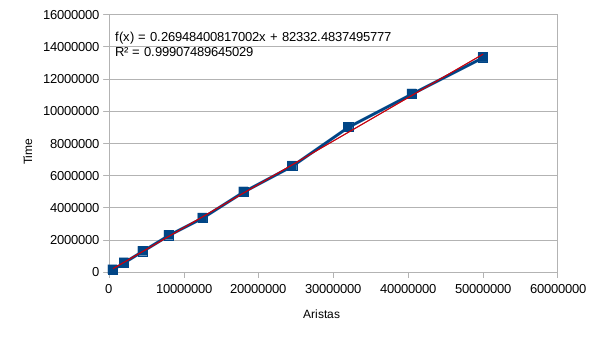
\includegraphics[scale=0.8]{kruskalPlot.png}
            \end{table}

            \newpage

            \small{\begin{lstlisting}
                vector<edge> kruskal(vector<vector<P>> adj)
                {
                    int n = adj.size();
                    double weight = 0;
                    int C[n], R[n];
                    vector <edge> T;
                    priority_queue <edge, vector <edge>> E;
                    
                    for(int i=0; i<n; ++i)// full anidated cilce O(E)
                    {
                        C[i] = i; R[i] = 0;
                        for (int j = 0; j < adj[i].size(); ++j)      
                            E.push(edge(i,adj[i][j].second, adj[i][j].first)); //O(log(E))
                    } //O(E*log(E))

                    while(T.size() < n-1 && !E.empty()) //O(E) worst case, empty pq (O(E))
                    {
                        edge cur = E.top(); E.pop(); //(O(log(E)))
                        int uc = find(C, cur.u), vc = find(C, cur.v); //alfa(v)
                        if(uc != vc)
                        {
                            T.push_back(cur); weight += cur.d;
                            if(R[uc] > R[vc]) C[vc] = uc;
                            else if(R[vc] > R[uc]) C[uc] = vc;
                            else { C[vc] = uc; R[uc]++; }
                        }
                    }
                    return T;
                } //O(E*(log(E) + log(v)))
            \end{lstlisting}} \normalsize

            Analizando el código podemos ver:
            \begin{itemize}
                \item La inicialización de la PQ y Unión-Find toma $\mathcal{O}(E\cdot log_2(E))$.
                \item La creación del MSD cuesta $\mathcal{O}(E\cdot ( log_2(E) + \alpha(V))$.
                \item Entonces tenemos que nos cuesta $\mathcal{O}(2E\cdot log_2(E) + E\cdot \alpha(V))$.
                \item $\therefore \mathcal{O}(E\cdot log_2(E))$.
            \end{itemize}
            
            Si vemos nuestro gráfico tiene forma de $x\cdot log(x)$, pero no podemos afirmar nada sin antes analizarlo.
            
            Observando su linea de tendencia podemos observar:

            \begin{itemize}
                \item La tendencia roja es lineal y fácilmente va a ser una cota inferior.
                \item De aquí podemos decir que tenemos $\Theta(x)$.
                \item Como sabemos que nuestro tiempo teórico es $\mathcal{O}(x\cdot log_2(x))$ confirmemos que se cumpla el punto anterior.
                \item $\lim_{x \to \infty} \frac{x}{x\cdot log_2(x)} = 0 \therefore$ Se concluye que es $\mathcal{O}(x\cdot log_2(x))$.
            \end{itemize}
           
        \newpage 
        \subsection{Dijkstra}
            \begin{table}[h]
                \centering
                \begin{tabular}{|c|c|c|c|}
                \hline
                Nodos  & Aristas  & Densidad & Tiempo     \\ \hline
                1000   & 499500   & 1        & 288138.5   \\ \hline
                2000   & 1999000  & 1        & 1685811.8  \\ \hline
                3000   & 4498500  & 1        & 4526754.8  \\ \hline
                4000   & 7998000  & 1        & 8534128.3  \\ \hline
                5000   & 12497500 & 1        & 14592132.5 \\ \hline
                6000   & 17997000 & 1        & 25031167.5 \\ \hline
                7000   & 24496500 & 1        & 35609440.9 \\ \hline
                8000   & 31996000 & 1        & 48022693.7 \\ \hline
                9000   & 40495500 & 1        & 61493204.6 \\ \hline
                10000  & 49995000 & 1        & 77250844.2 \\ \hline
                \end{tabular}
                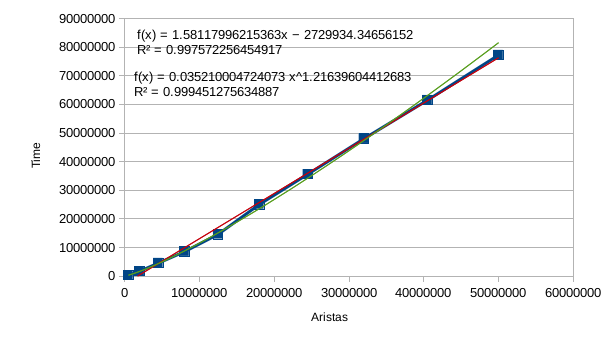
\includegraphics[scale=0.8]{dijkstraPlot.png}
            \end{table}

            \small{\begin{lstlisting}
                vector<int> dijkstra(vector<vector<P>> edges, int s, int t)
                {
                    priority_queue<P, vector<P>, greater<P> > Q;
                    vector<double> dist(edges.size(), INF); vector<int> dad(edges.size(), -1);
                    Q.push (make_pair (0, s)); dist[s] = 0;
                    while (!Q.empty())  //pq + for O(E+V)
                    {
                        P p = Q.top(); Q.pop();
                        if (p.second == t) break;
                        int here = p.second;
                        for (int i = 0; i< edges[here].size(); ++i) 
                        {
                            if (dist[here] + edges[here][i].first < dist[edges[here][i].second])
                            {
                                dist[edges[here][i].second] = dist[here] + edges[here][i].first;
                                dad[edges[here][i].second] = here;
                                Q.push (make_pair (dist[edges[here][i].second], edges[here][i].second)); //O(Log(v)) 
                            }
                        }
                    } //O(E+V(Log(V)))
                    return dad;
                }
            \end{lstlisting}} \normalsize

            Analizando el código podemos ver:
            \begin{itemize}
                \item Realizar todo el ciclo anidado cuesta $\mathcal{O}(E+V)$.
                \item La extracción de la PQ cuesta $\mathcal{O}(log_2(V))$.
                \item Tenemos $\mathcal{O}((E+V)\cdot log_2(v))$.
                \item Como es un grafo conexo sabemos que $E \geq V-1 \implies \mathcal{O}(2E\cdot log_2(v))$.
                \item $\therefore \mathcal{O}(E\cdot log_2(v))$.
            \end{itemize}

            Si vemos nuestro gráfico tiene forma de $x\cdot log(x)$ pero no podemos afirmar nada sin antes analizarlo y como sabemos que nuestro tiempo teórico es de $\mathcal{O}(E\cdot log_2(v))$ como no podemos analizar dos variables en nuestro gráfico y sabemos que $E \geq V-1$ por simplicidad aceptaremos el error de decir que nuestra complejidad es de $\mathcal{O}(E\cdot log_2(E))$.
        
            Observando su línea de tendencia podemos observar:

            \begin{itemize}
                \item La tendencia verde no es mayor que $x^{1.2}$ y fácilmente va a ser una cota superior.
                \item La tendencia roja es lineal y fácilmente va a ser una cota inferior.
                \item De aquí podemos decir que tenemos $\Theta(x) \land \Omega(x^{1.2})$.
                \item Como sabemos que nuestro tiempo teórico es $\mathcal{O}(x\cdot log_2(x))$ confirmemos que se cumpla el punto anterior.
                \item $\lim_{x \to \infty} \frac{x^{1.2}}{x\cdot log_2(x)} = \infty \land \lim_{x \to \infty} \frac{x}{x\cdot log_2(x)} = 0$.
                \item $\therefore$ Utilizando el teorema del sandwich se concluye que es  $\mathcal{O}(x\cdot log_2(x))$.
            \end{itemize}
        
        \section{Conclusión}
            Gracias a este trabajo, logré aprender bastante de grafos y cómo implementar sus algoritmos icónicos. También puse en práctica nuevas estructuras las cuales no había utilizado antes.
            Por último, también se obtuvieron los resultados esperados de este experimento sin ninguna mayor dificultad, salvo algunos errores menores que luego se corrigeron sin problemas.

        \section{Anexos}
            \href{https://users.dcc.uchile.cl/~raparede/publ/08PhDthesis.pdf}{Grafos para búsqueda en espacios métricos} Rodrigo Paredes Moraleda 

            \href{https://users.dcc.uchile.cl/~raparede/publ/08PhDthesis.pdf}{https://users.dcc.uchile.cl/~raparede/publ/08PhDthesis.pdf}
            
            \bigskip
            Como adjunto, también se encuentra un archivo excel que contiene más detalles sobre los tiempos del experimento.

            %\bigskip
            %Agradecimientos al "Sofá"... y \href{https://www.stackoverflow.com}{StackOverflow}
            
\end{document}
